\documentclass[dvipsnames,
%xcolor={svgnames},
hyperref={
	citecolor=blue,
	colorlinks=true,
	urlcolor=blue,
	linkcolor=,
}
]{beamer}
\beamertemplatenavigationsymbolsempty
\usetheme{Boadilla}
\usefonttheme[onlymath]{serif}

\usepackage{cleveref}

\usepackage{amsmath}
\usepackage{bm}
\usepackage{bbm}
\usepackage{mathrsfs}
\usepackage{mathtools}
\usepackage[cal=boondoxo]{mathalpha}

% Change horizontal spacing
\setlength{\tabcolsep}{3pt}

\usepackage[none]{hyphenat} % no hyphenation

\usepackage{array}

\usepackage{cancel}

\usepackage[style=authoryear,maxcitenames=2,backend=biber,citetracker=true]{biblatex}
\addbibresource{references.bib}

\usepackage{verbatim}

\usepackage{bigints}

\usepackage{makecell}

\usepackage{subcaption}

\usepackage{booktabs}

\colorlet{darkgreen}{green!65!black}

\DeclareCiteCommand{\citeauthor}
{\boolfalse{citetracker}%
	\boolfalse{pagetracker}%
	\usebibmacro{prenote}}
{\ifciteindex
	{\indexnames{labelname}}
	{}%
	\printtext[bibhyperref]{\printnames{labelname}}}
{\multicitedelim}
{\usebibmacro{postnote}}

\DeclareCiteCommand{\citeyear}
{\usebibmacro{prenote}}
{\bibhyperref{\printfield{year}}\bibhyperref{\printfield{extrayear}}}
{\multicitedelim}
{\usebibmacro{postnote}}

\newcommand{\credit}[2]{{\par\hfill \tiny #1 credit:~\itshape{\color{blue} \citeauthor{#2} (\citeyear{#2})}}}
\newcommand{\crediturl}[2]{{\par\hfill \tiny #1 credit:~\itshape{\color{blue} \url{#2}}}}
\let\oldcite\cite
\renewcommand{\cite}[1]{{\color{blue} \oldcite{#1}}}
\newcommand{\citefoot}[1]{{\color{blue} \citeauthor{#1} (\citeyear{#1})}}
\newcommand{\matr}[1]{#1}

\newcommand{\red}[1]{{\color{red} #1}}

\title[Deep Imbalanced Regression]
{\href{https://doi.org/10.48550/arXiv.2102.09554}{Deep Imbalanced Regression}}
%\subtitle{}
\author[Yang Y. et al.]{Yang Y, Zha K, Chen Y, Wang H, Katabi D}
%\institute{Aalto University}
\date{}%3 July 2024}

\addtobeamertemplate{title page}{}{
\begin{center}
\vspace{-5em}
ICML 2021
\\\vspace{4em}Presenter: Gianmarco Midena
\\\vspace{1em}26 November 2024
\end{center}}

\begin{document}
	
\begin{frame}[noframenumbering,plain]
\titlepage
\end{frame}

\begin{frame}{Overview}
	\begin{figure}[h]
		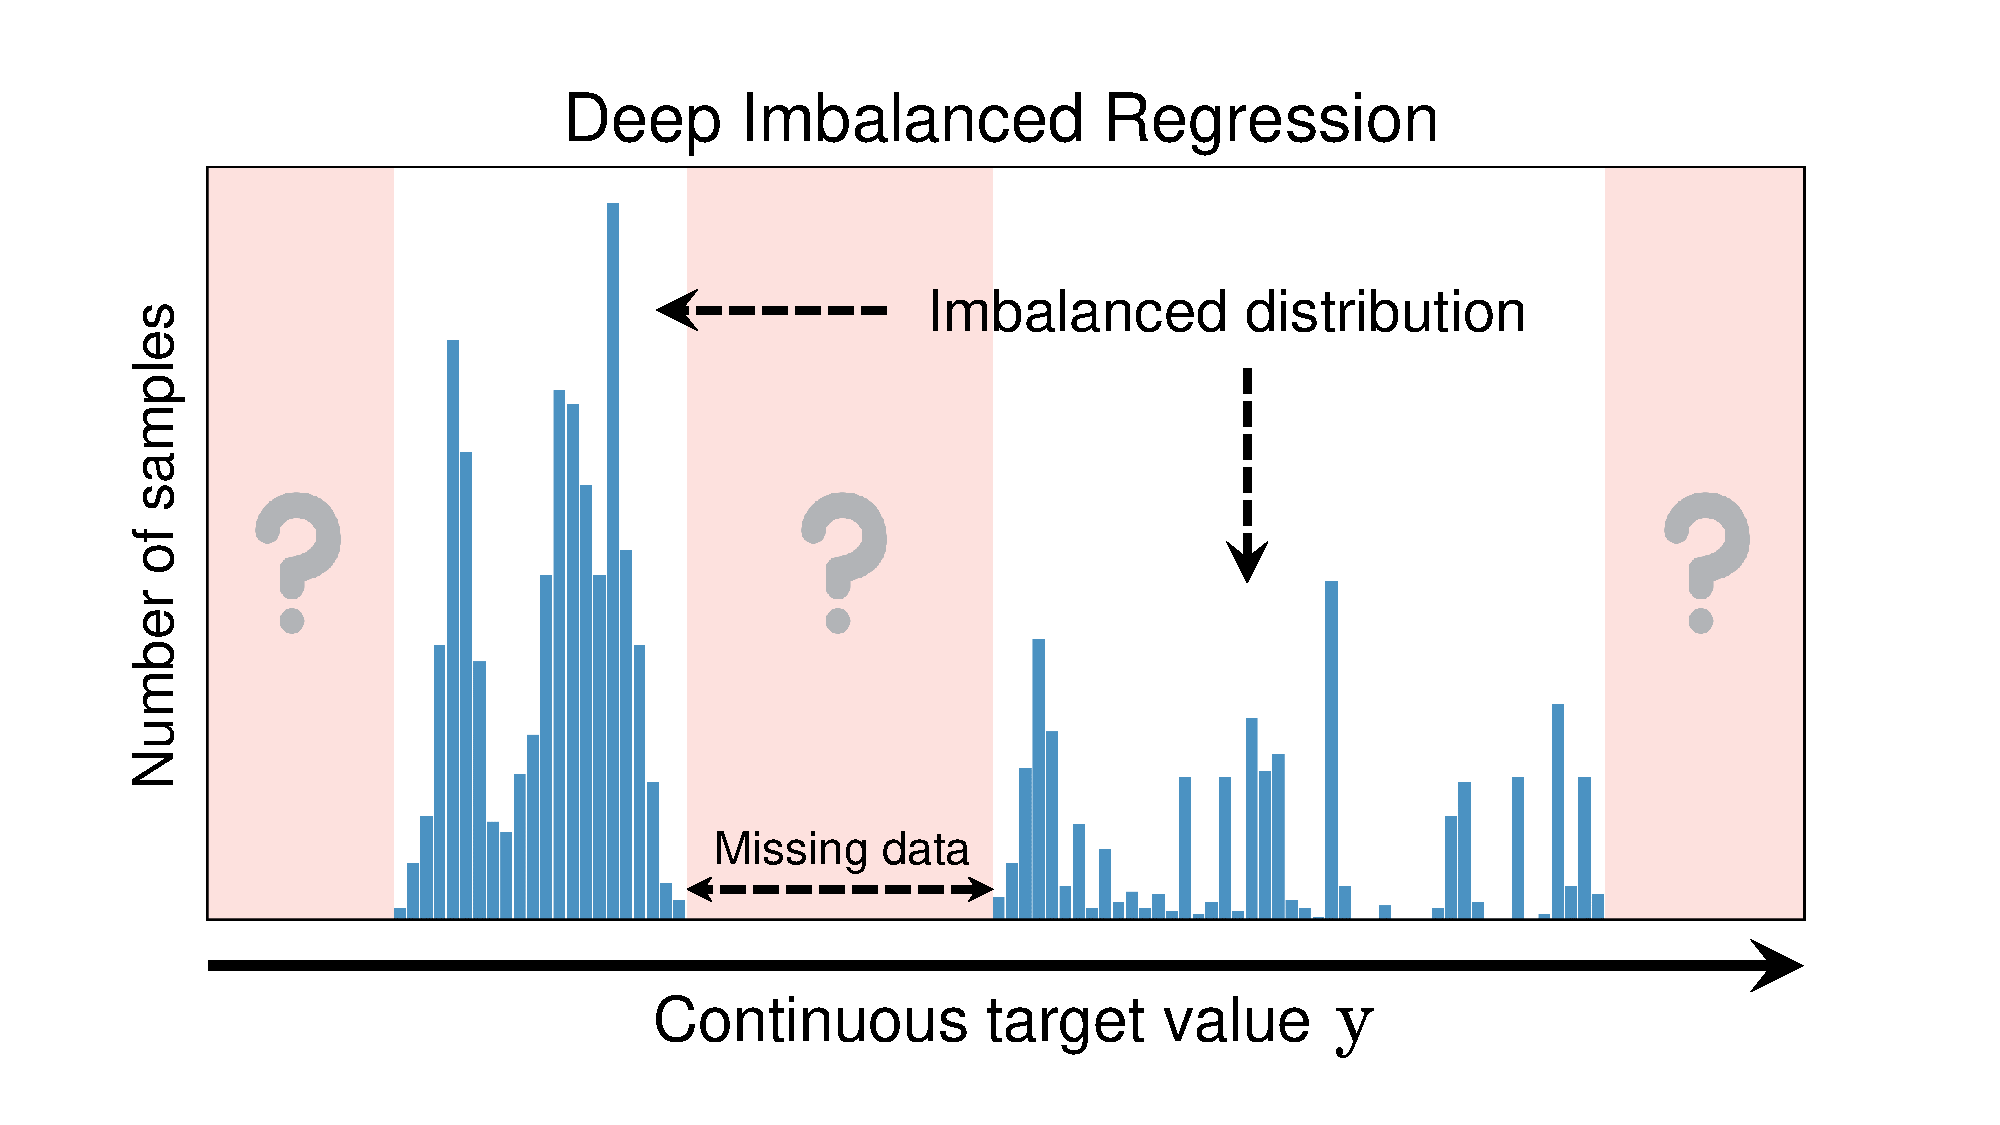
\includegraphics[width=\linewidth]{images/teaser.pdf}
		%\caption{}
	\end{figure}
	\credit{Image}{yang2021delving}
\end{frame}



\begin{frame}{Problem Settings}
	\begin{itemize}
		\item $\{(\mathbf{x}_i, y_i)\}_{i=1}^N$: training set
		\item $\mathbf{x}_i\in\mathbb{R}^{d}$: input
		\item $y_i\in\mathcal{Y}$: continuous label or target
		\item $b_i\in\mathcal{B}$: discrete label or target
		\item $\mathcal{Y}\subset\mathbb{R}$: continuous label space
		\item $\mathcal{B} = \{1,\dots,M\}\subset\mathbb{Z}^+$: index space
		\begin{itemize}
			\item divides $\mathcal{Y}$ into $M$ groups (bins) with equal intervals $[t_j, t_{j+1})$
			\item $\{[t_0, t_1), \dots, [t_{M-1}, t_M)\}$: discrete label space
			\item $t_k\in\mathcal{Y}$
			\item minimum resolution
			\begin{itemize}
				\item e.g., $\delta y \triangleq t_{j+1} - t_j = 1$ in age estimation
			\end{itemize}	
		\end{itemize}
		\item $\hat{y}_i = g(\mathbf{z}_i) \in \mathbb{R}$: predicted continuous label
		\item $\mathbf{z}_i = f(\mathbf{x}_i; \theta) \in \mathbb{R}^{d'}$: learned representation
		\item $\theta$: trainable model parameters
	\end{itemize}
\end{frame}

\begin{frame}{Evaluation}
	\begin{itemize}\setlength\itemsep{1.5em}
		\item Divide target space into disjoint regions (bins)
		\begin{itemize}
			\item \emph{Many-shot}: $>100$ training examples
			\item \emph{Medium-shot}: $20$-$100$ training examples
			\item \emph{Few-shot}: $<20$ training examples
			\item \emph{Zero-shot}: $0$ training examples
			\item[-] Inspired by \cite{liu2019large}
		\end{itemize}
		\item Metrics
		\begin{itemize}
			\item Mean Absolute Error (MAE)
			\item Mean Squared Error (MSE)
			\item Pearson Correlation (PCC)
			\item Geometric Mean Error (GME)
			\begin{equation*}
				GME = \sqrt[n]{\prod_{i=1}^n |y_i - \hat{y_i}|}
			\end{equation*}
			\begin{itemize}
				\item Pros: + fairness (uniformity) in prediction
			\end{itemize}
		\end{itemize}
	\end{itemize}
\end{frame}

\begin{frame}{(Training) Datasets - Label Distributions}
	\begin{center}
		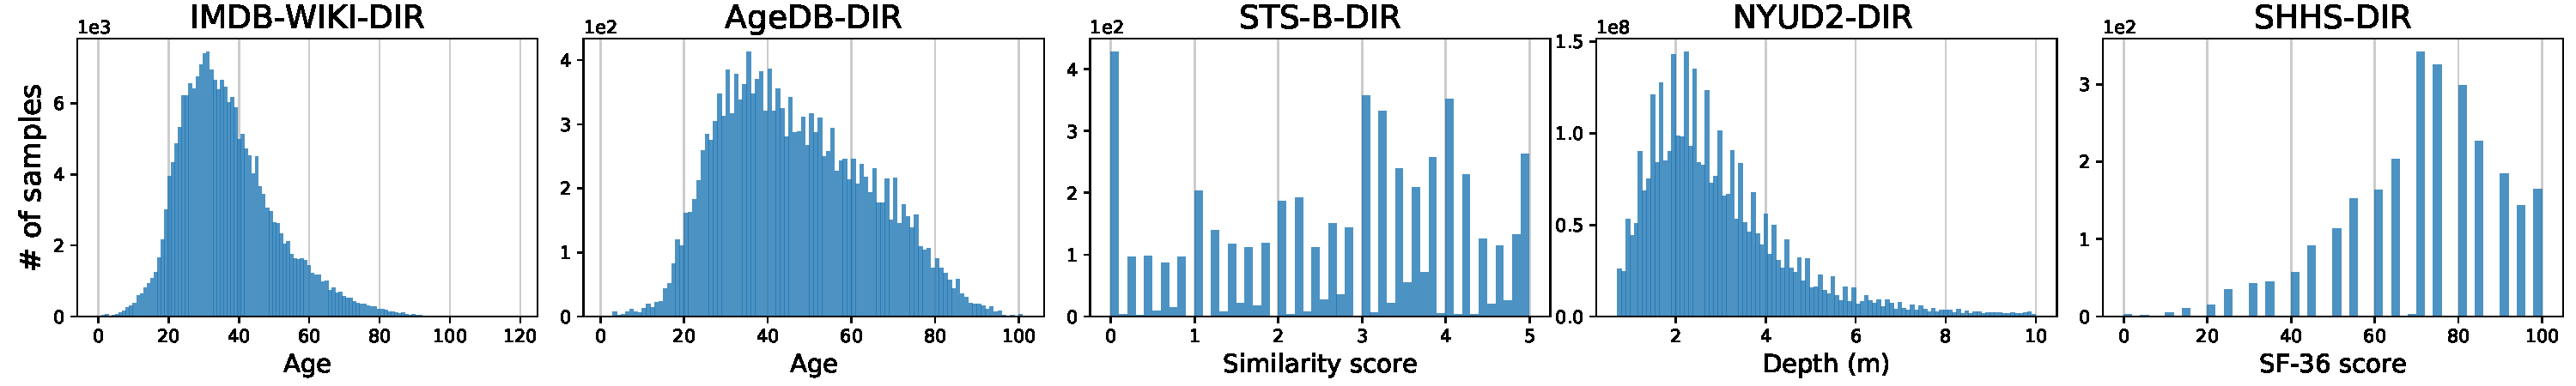
\includegraphics[trim={0 0 52em 0},clip,scale=0.4]{images/dataset_info.pdf}
		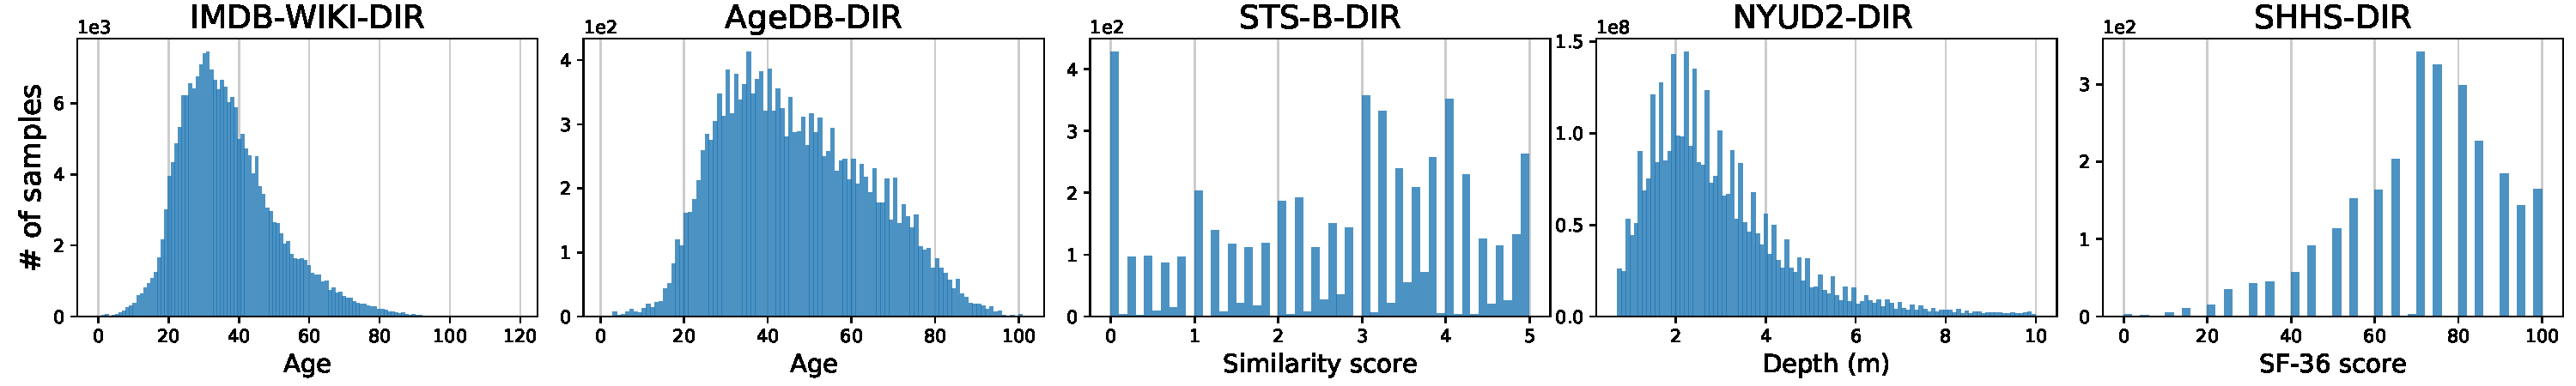
\includegraphics[trim={78.8em 0 0 0},clip,scale=0.4]{images/dataset_info.pdf}
	\end{center}
	\credit{Image}{yang2021delving}
\end{frame}

\begin{frame}{Test Error on Categorical vs. Continuous Label Space}
	\begin{figure}[h]
	\begin{subfigure}{0.48\textwidth}
		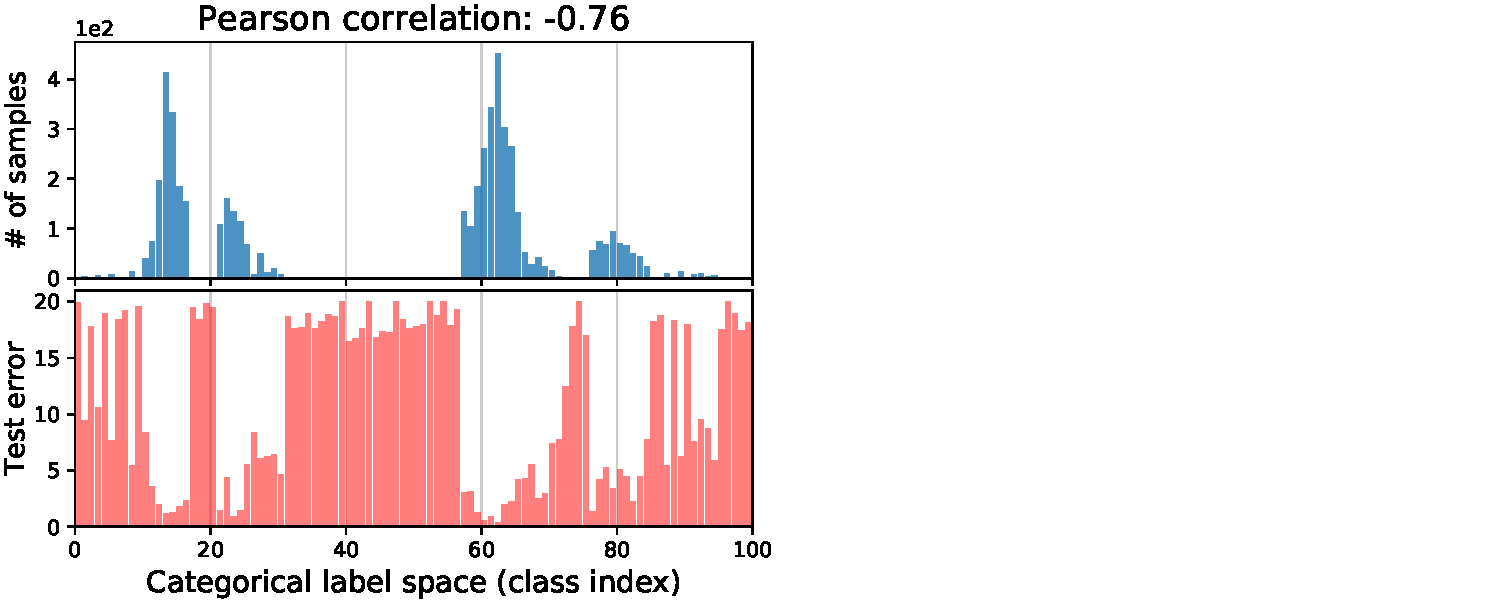
\includegraphics[width=\linewidth]{images/err_motivate_1_left.pdf}
		\caption{CIFAR-100 (subsampled)}
	\end{subfigure}\hspace{1em}%
	\begin{subfigure}{0.48\textwidth}
		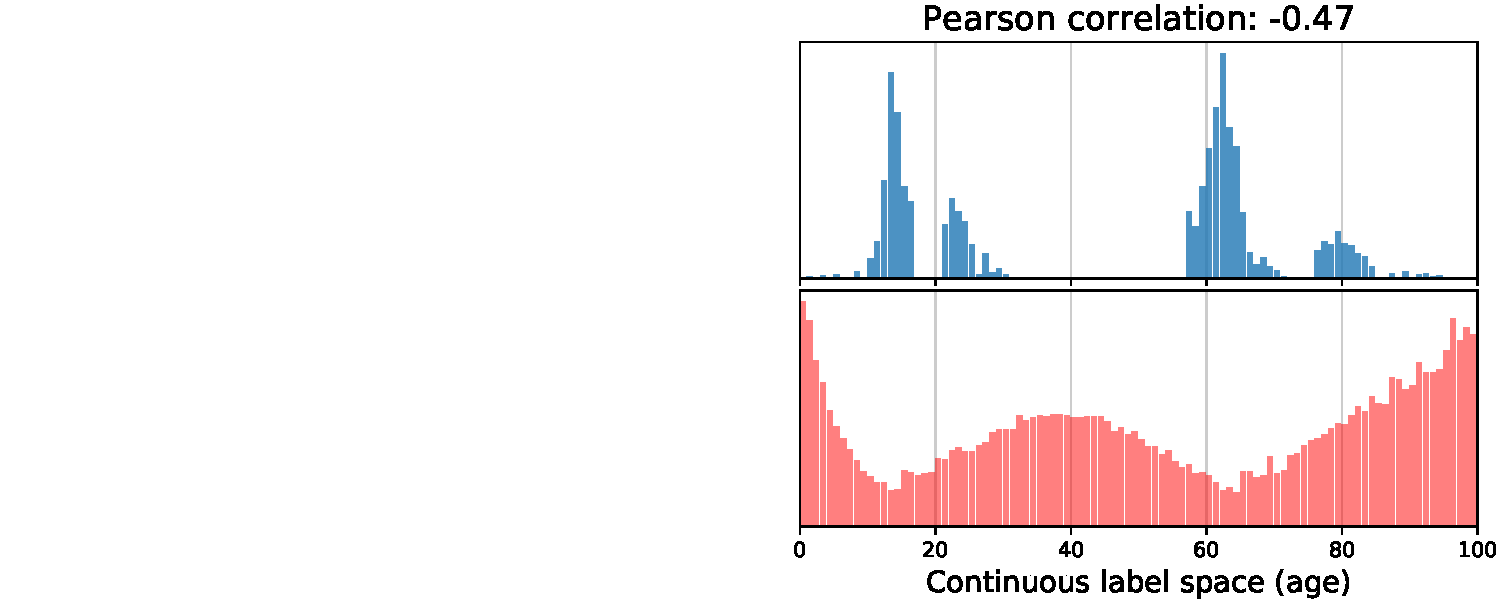
\includegraphics[width=\linewidth]{images/err_motivate_1_right.pdf}
		\caption{IMDB-WIKI (subsampled)}
	\end{subfigure}
	%\caption{}
	\end{figure}
	\credit{Image}{yang2021delving}
\end{frame}

\begin{frame}{Label Distribution Smoothing}
	\begin{figure}[h]
		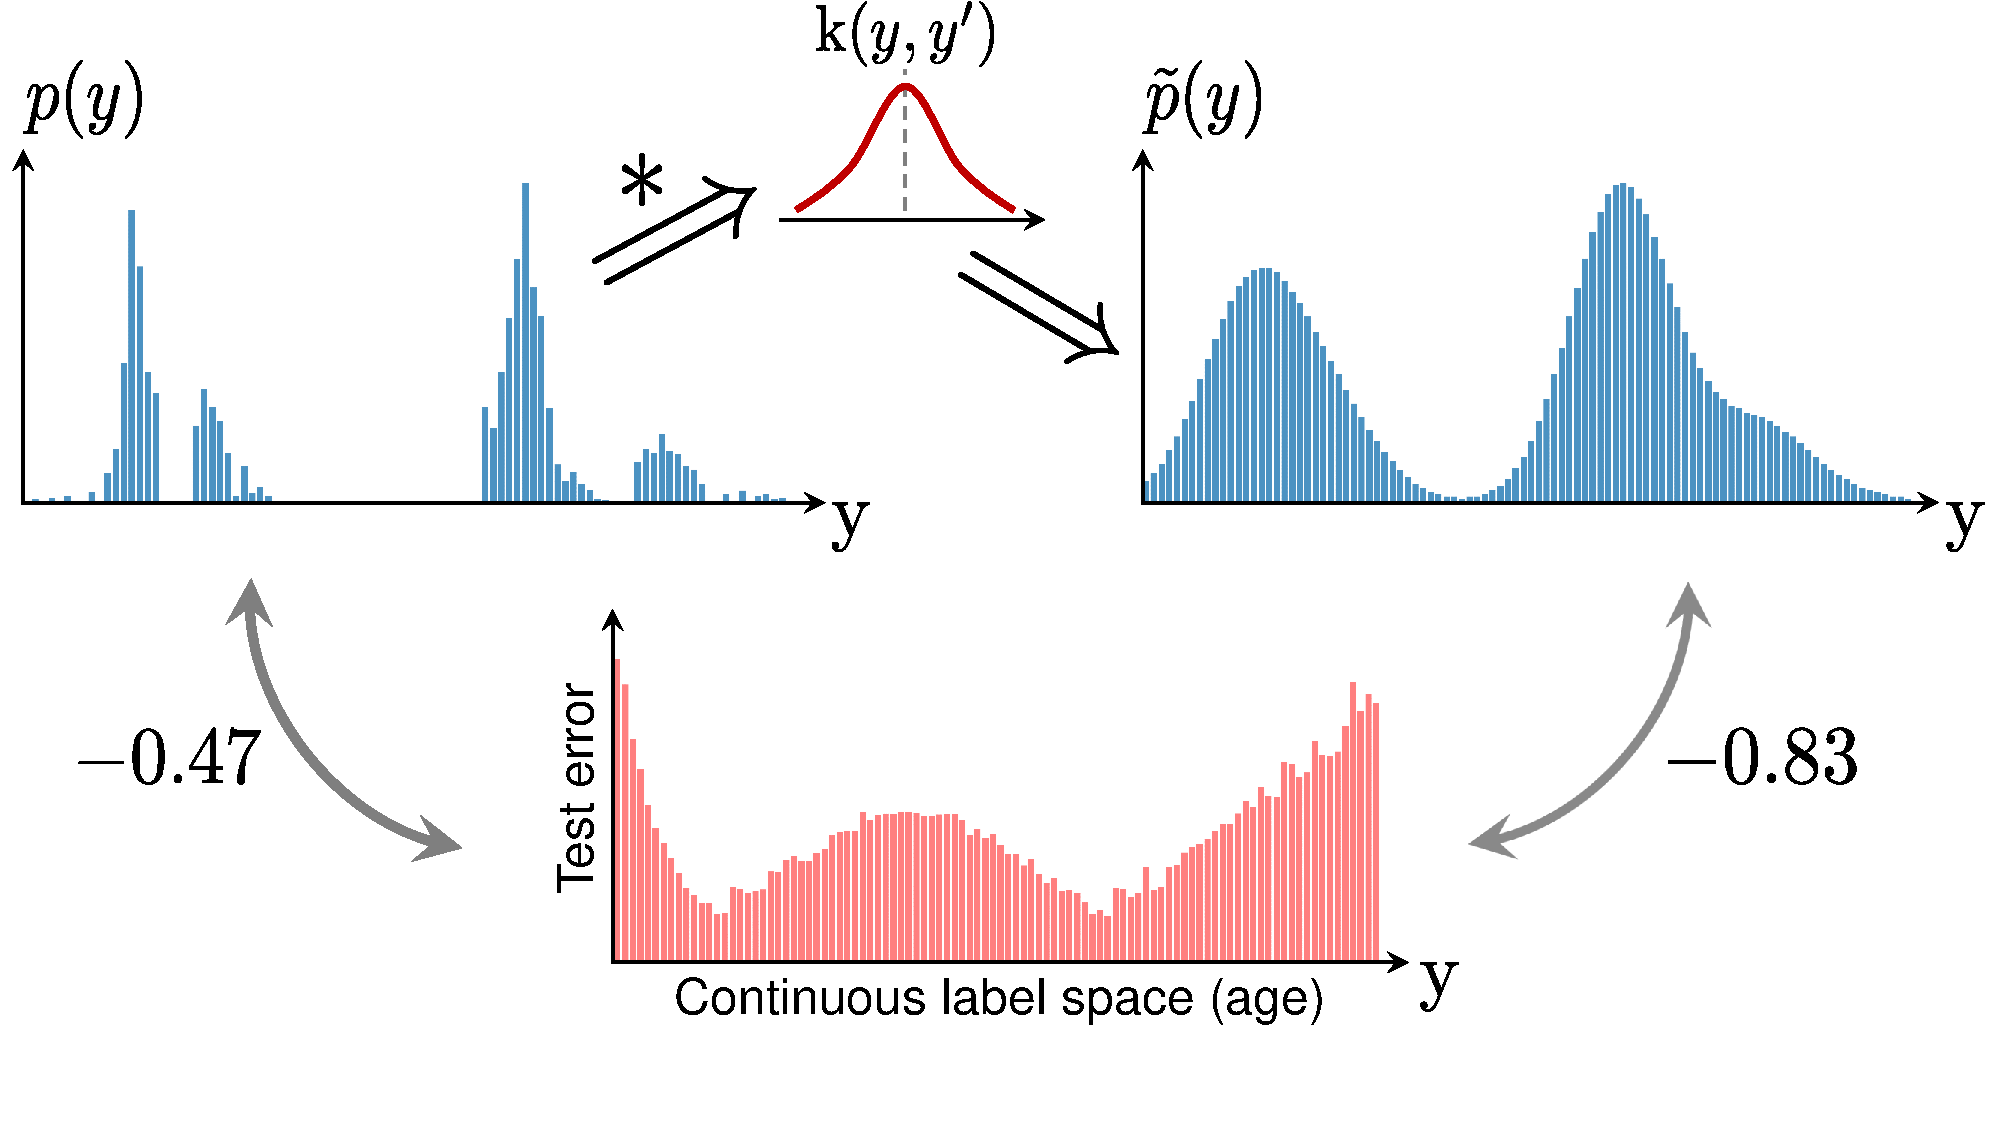
\includegraphics[width=\linewidth]{images/err_motivate_sep.pdf}
		%\caption{}
	\end{figure}
	\credit{Image}{yang2021delving}
\end{frame}

\begin{frame}{Feature Distribution Smoothing}
	\begin{figure}[h]
		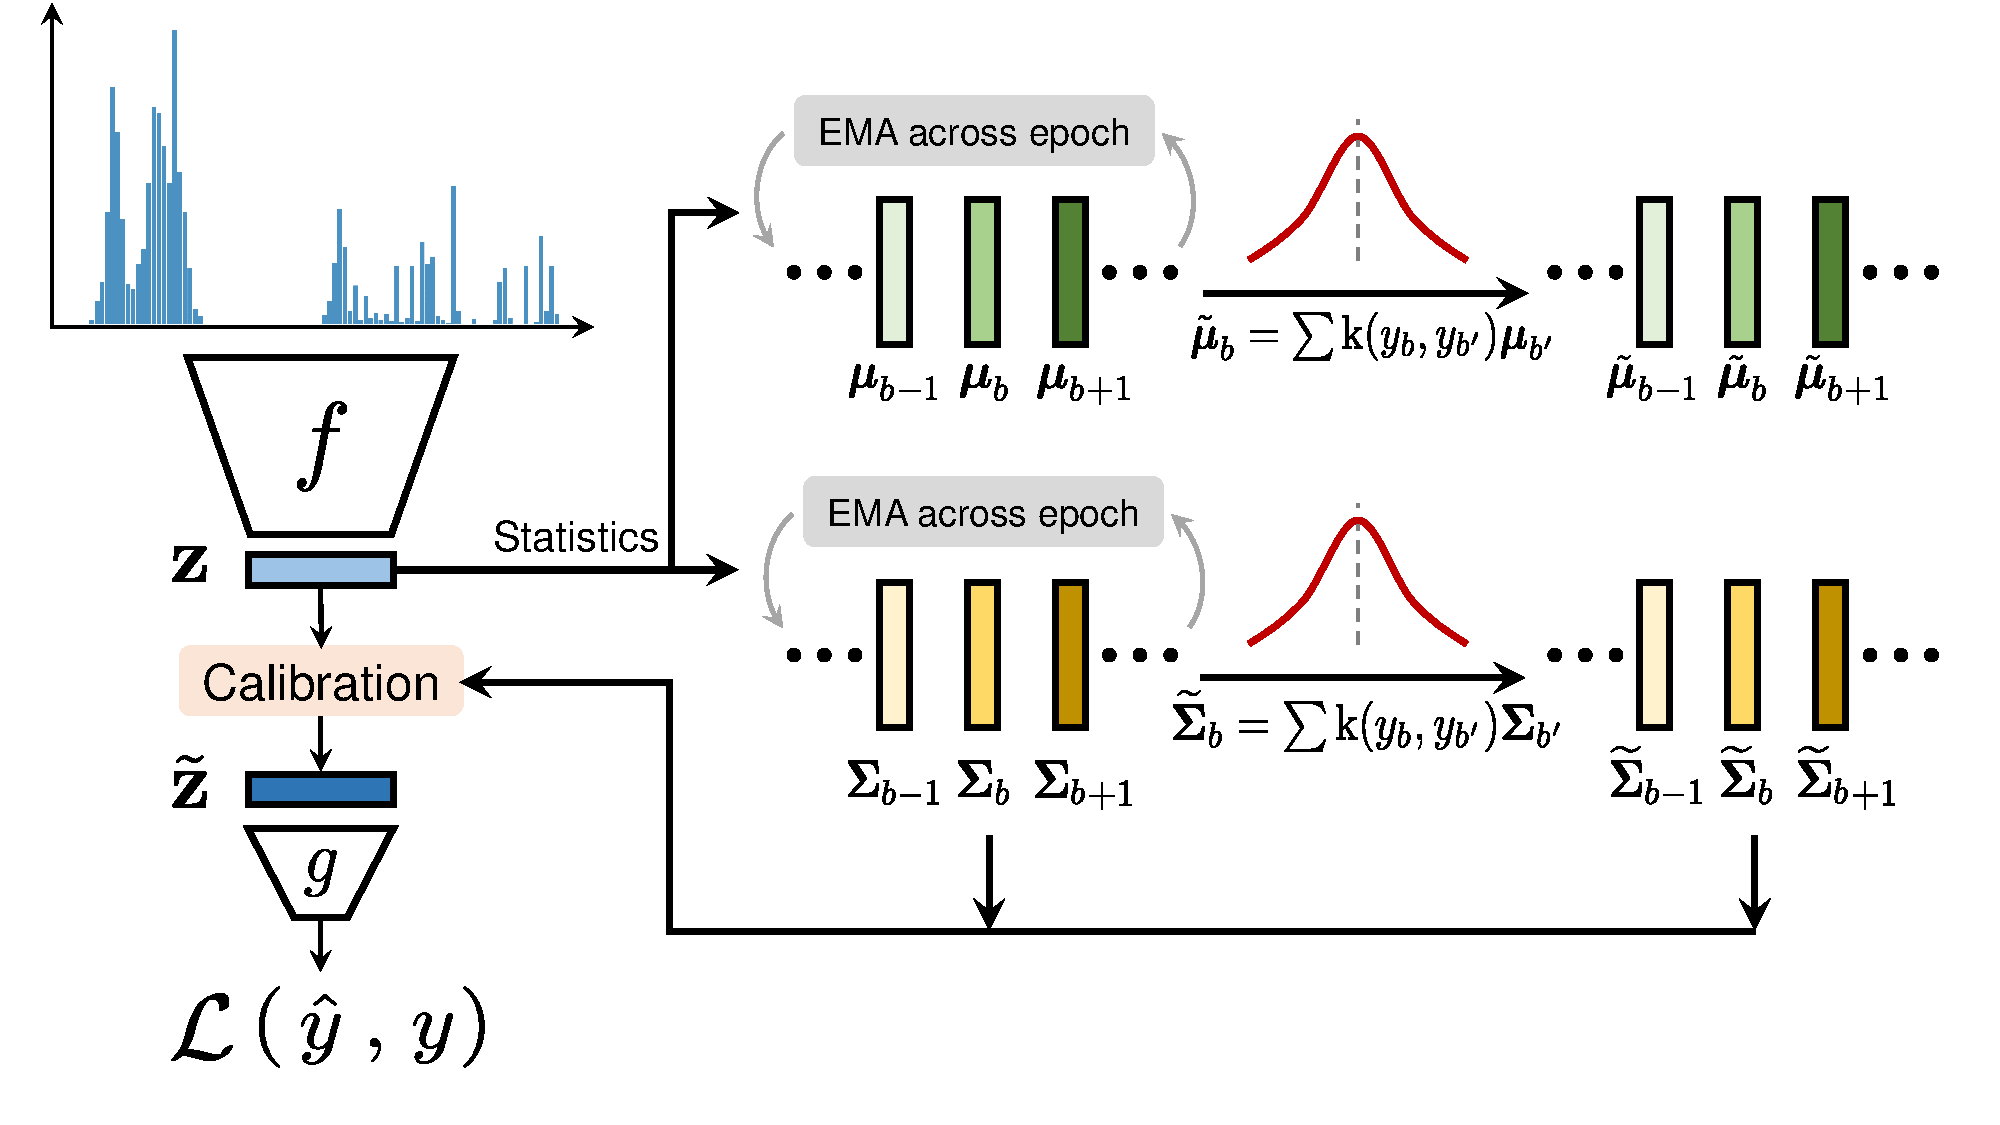
\includegraphics[width=\linewidth]{images/teaser_fds.pdf}
		%\caption{}
	\end{figure}
	\credit{Image}{yang2021delving}
\end{frame}

\begin{frame}{Baselines (1/2)}
	\begin{enumerate}\setlength\itemsep{1.5em}
		\item<1-> Vanilla: neglects data imbalance
		\item<2-> Synthetic samples
		\begin{itemize}
			\item SMOTER (\cite{torgo2013smote})
			\begin{enumerate}
				\item Defines frequent and rare regions using label density.
				\item Creates synthetic samples for pre-defined rare regions by linearly interpolating both inputs and labels.
			\end{enumerate}
			\item SMOGN (\cite{branco2017smogn}): augments SMOTER with Gaussian noise
		\end{itemize}
		\item<3-> Focal-R
		\begin{equation*}
			\frac{1}{n} \sum_{i=1}^n \sigma(|\beta e_i|)^\gamma e_i
		\end{equation*}
		\begin{itemize}
			\item Error-aware loss
			\item Maps absolute error into $[0, 1]$.
			\item $e_i$: $L_1$ error for $i$-th sample
			\item $\beta$, $\gamma$: hyper-parameters
			\item Inspired by Focal Loss (\cite{lin2017focal}) for classification
		\end{itemize}
	\end{enumerate}
\end{frame}

\begin{frame}{Baselines (2/2)}
	\begin{enumerate}\setcounter{enumi}{3}\setlength\itemsep{1.5em}
		\item<1-> Regressor re-training (RRT)
		\begin{itemize}
			\item Two-stage training
			\begin{enumerate}
				\item Train encoder
				\item Re-train regressor with inverse re-weighting and frozen encoder.
			\end{enumerate}
			\item Inspired by \cite{kang2019decoupling}
		\end{itemize}
		\item<2-> Cost-sensitive re-weighting: re-weighting schemes based on label distribution
		\begin{itemize}
			\item Inverse-frequency weighting (INV)
			\item Square-root weighting variant (SQINV)
		\end{itemize}
	\end{enumerate}
\end{frame}

\sectionframe{Results}

\begin{frame}{Inferring Age from Images}{IMDB-WIKI}
	\begin{table}[t]
		\setlength{\tabcolsep}{2.5pt}
		\small
		\begin{center}
			\resizebox{0.6\textwidth}{!}{
				\begin{tabular}{l|cccc|cccc}
					\toprule[1.5pt]
					Metrics      & \multicolumn{4}{c|}{MAE~$\downarrow$}     & \multicolumn{4}{c}{GM~$\downarrow$}  \\ \midrule
					Shot         & All  & Many & Med. & Few   & All  & Many & Med. & Few   \\ \midrule\midrule
					\textsc{Vanilla}      & 8.06 & 7.23 & 15.12  & 26.33 & 4.57 & 4.17 & 10.59  & 20.46 \\ \midrule\midrule
					\textsc{SmoteR}~(\cite{torgo2013smote})       & 8.14 & 7.42 & 14.15  & 25.28 & 4.64 & \textbf{4.30} & 9.05   & 19.46 \\[1.2pt]
					\textsc{SMOGN}~(\cite{branco2017smogn})        & 8.03 & \textbf{7.30} & 14.02  & 25.93 & 4.63 & \textbf{4.30} & 8.74   & 20.12 \\[1.2pt]
					\textsc{SMOGN} + \textbf{\textsc{LDS}}   & 8.02 & 7.39 & 13.71 & 23.22 & 4.63 & 4.39 & 8.71 & 15.80 \\[1.2pt]
					\textsc{SMOGN} + \textbf{\textsc{FDS}}   & 8.03 & 7.35 & 14.06 & 23.44 & 4.65 & 4.33 & 8.87 & 16.00 \\[1.2pt]
					\textsc{SMOGN} + \textbf{\textsc{LDS}} + \textbf{\textsc{FDS}}   & \textbf{7.97} & 7.38 & \textbf{13.22} & \textbf{22.95} & \textbf{4.59} & 4.39 & \textbf{7.84} & \textbf{14.94} \\ \midrule\midrule
					\textsc{Focal-R}      & 7.97 & 7.12 & 15.14  & 26.96 & 4.49 & 4.10 & 10.37  & 21.20 \\[1.2pt]
					\textsc{Focal-R} + \textbf{\textsc{LDS}} & {7.90}  & \textbf{7.10}  &  14.72   & 25.84  & \textbf{4.47}   & \textbf{4.09}    & {10.11}     & {19.14}     \\[1.2pt]
					\textsc{Focal-R} + \textbf{\textsc{FDS}}   & 7.96 & 7.14 & 14.71 & 26.06 & 4.51 & 4.12 & 10.16 & 19.56 \\[1.2pt]
					\textsc{Focal-R} + \textbf{\textsc{LDS}} + \textbf{\textsc{FDS}}   & \textbf{7.88} & \textbf{7.10} & \textbf{14.08}  & \textbf{25.75}   & \textbf{4.47} & 4.11 & \textbf{9.32} & \textbf{18.67} \\ \midrule\midrule
					\textsc{RRT}          & 7.81 & 7.07 & 14.06  & 25.13 & 4.35 & 4.03 & 8.91   & 16.96 \\[1.2pt]
					\textsc{RRT} + \textbf{\textsc{LDS}} & {7.79} &  7.08  & {13.76}  & {24.64} & {4.34} & \textbf{4.02} & {8.72} & {16.92} \\[1.2pt]
					\textsc{RRT} + \textbf{\textsc{FDS}}   & \textbf{7.65}  & \textbf{7.02} & 12.68 & 23.85 & \textbf{4.31} & 4.03 & 7.58 & 16.28 \\[1.2pt]
					\textsc{RRT} + \textbf{\textsc{LDS}} + \textbf{\textsc{FDS}}   & \textbf{7.65}  & 7.06  & \textbf{12.41}  & \textbf{23.51}  & \textbf{4.31} & {4.07} & \textbf{7.17} & \textbf{15.44} \\ \midrule\midrule
					\textsc{SQInv}      & 7.87 & 7.24 & 12.44  & 22.76 & 4.47 & 4.22 & 7.25   & 15.10 \\[1.2pt]
					\textsc{SQInv} + \textbf{\textsc{LDS}} & {7.83} & 7.31 & \textbf{12.43}  & {22.51} & {4.42} & {4.19} & {7.00}  & {13.94} \\[1.2pt]
					\textsc{SQInv} + \textbf{\textsc{FDS}}   & 7.83 & 7.23 & 12.60  & 22.37  & 4.42 & 4.20 & \textbf{6.93} & 13.48  \\[1.2pt]
					\textsc{SQInv} + \textbf{\textsc{LDS}} + \textbf{\textsc{FDS}}   & \textbf{7.78} & \textbf{7.20} & {12.61} & \textbf{22.19} & \textbf{4.37}    & \textbf{4.12} & 7.39  & \textbf{12.61}  \\ \midrule\midrule
					\textsc{\textbf{Ours~(best)} vs. Vanilla}   & \textcolor{darkgreen}{\textbf{+0.41}} & \textcolor{darkgreen}{\textbf{+0.21}} & \textcolor{darkgreen}{\textbf{+2.71}} & \textcolor{darkgreen}{\textbf{+4.14}} & \textcolor{darkgreen}{\textbf{+0.26}} & \textcolor{darkgreen}{\textbf{+0.15}} & \textcolor{darkgreen}{\textbf{+3.66}} & \textcolor{darkgreen}{\textbf{+7.85}} \\
					\bottomrule[1.5pt]
				\end{tabular}
			}
		\end{center}
	\end{table}
	\begin{itemize}\fontsize{7pt}{7.2}\selectfont
		\item Either LDS, FDS, or both leads to performance gains.
		\item LDS + FDS often achieves the best results:
		\begin{itemize}\fontsize{7pt}{7.2}\selectfont
			\item maintains or improves performance overall
			and on many-shot regions,
			\item boosts performance for medium-shot and few-shot regions.
		\end{itemize}
	\end{itemize}
	\credit{Table}{yang2021delving}
\end{frame}

\begin{frame}{Inferring Age from Images}{AgeDB}
	\begin{table}[t]
		\setlength{\tabcolsep}{2.5pt}
		\small
		\begin{center}
			\resizebox{0.6\textwidth}{!}{
				\begin{tabular}{l|cccc|cccc}
					\toprule[1.5pt]
					Metrics      & \multicolumn{4}{c|}{MAE~$\downarrow$}     & \multicolumn{4}{c}{GM~$\downarrow$}  \\ \midrule
					Shot         & All  & Many & Med. & Few   & All  & Many & Med. & Few   \\ \midrule\midrule
					\textsc{Vanilla}      & 7.77 & 6.62 & 9.55   & 13.67 & 5.05 & 4.23 & 7.01   & 10.75 \\ \midrule\midrule
					\textsc{SmoteR}~(\cite{torgo2013smote})       & 8.16  & 7.39   & 8.65 & 12.28 & 5.21    & 4.65    & 5.69 & 8.49    \\[1.2pt]
					\textsc{SMOGN}~(\cite{branco2017smogn})        & 8.26  & 7.64   & 9.01 & 12.09 & 5.36    & 4.90    & 6.19 & 8.44    \\[1.2pt]
					\textsc{SMOGN} + \textbf{\textsc{LDS}}   & 7.96 & 7.44 & 8.64  & 11.77 & 5.03 & 4.68 & 5.69  & 7.98  \\[1.2pt]
					\textsc{SMOGN} + \textbf{\textsc{FDS}}   & 8.06 & 7.52 & 8.75  & 11.89 & 5.02 & 4.66 & 5.63  & 8.02  \\[1.2pt]
					\textsc{SMOGN} + \textbf{\textsc{LDS}} + \textbf{\textsc{FDS}}   & \textbf{7.90} & \textbf{7.32}  & \textbf{8.51}  & \textbf{11.19}  & \textbf{4.98}  & \textbf{4.64}  & \textbf{5.41} & \textbf{7.35} \\ \midrule\midrule
					\textsc{Focal-R}      & 7.64 & 6.68 & 9.22   & 13.00 & 4.90 & 4.26 & 6.39   & 9.52  \\[1.2pt]
					\textsc{Focal-R} + \textbf{\textsc{LDS}}      & 7.56 & \textbf{6.67} & 8.82   & 12.40 & 4.82 & 4.27 & 5.87   & 8.83  \\[1.2pt]
					\textsc{Focal-R} + \textbf{\textsc{FDS}}      & 7.65 & 6.89 & 8.70   & \textbf{11.92} & 4.83 & 4.32 & 5.89   & \textbf{8.04}  \\[1.2pt]
					\textsc{Focal-R} + \textbf{\textsc{LDS}} + \textbf{\textsc{FDS}} & \textbf{7.47} & 6.69 & \textbf{8.30}  & 12.55 & \textbf{4.71} & \textbf{4.25} & \textbf{5.36}  & 8.59  \\ \midrule\midrule
					\textsc{RRT}          & 7.74 & 6.98 & 8.79   & 11.99 & 5.00 & 4.50 & 5.88   & 8.63  \\[1.2pt]
					\textsc{RRT} + \textbf{\textsc{LDS}}     & {7.72} & 7.00 & {8.75}   & {11.62} & {4.98} & 4.54 & {5.71}   & {8.27}  \\[1.2pt]
					\textsc{RRT} + \textbf{\textsc{FDS}}     & {7.70} & \textbf{6.95} & {8.76}   & {11.86} & {4.82} & \textbf{4.32} & {5.83}   & {8.08}  \\[1.2pt]
					\textsc{RRT} + \textbf{\textsc{LDS}} + \textbf{\textsc{FDS}}     & \textbf{7.66} & 6.99 & \textbf{8.60}   & \textbf{11.32} & \textbf{4.80} & 4.42 & \textbf{5.53}   & \textbf{6.99}  \\ \midrule\midrule
					\textsc{SQInv}      & 7.81 & 7.16 & 8.80   & 11.20 & 4.99 & 4.57 & 5.73   & 7.77  \\[1.2pt]
					\textsc{SQInv} + \textbf{\textsc{LDS}} & 7.67 & \textbf{6.98} & 8.86   & 10.89 & 4.85 & {4.39} &  5.80  & {7.45}  \\[1.2pt]
					\textsc{SQInv} + \textbf{\textsc{FDS}} & 7.69 & 7.10 & 8.86   & \textbf{9.98} & 4.83 & {4.41} &  5.97  & \textbf{6.29}  \\[1.2pt]
					\textsc{SQInv} + \textbf{\textsc{LDS}} + \textbf{\textsc{FDS}} & \textbf{7.55} &  7.01  & \textbf{8.24}   & 10.79 & \textbf{4.72} & \textbf{4.36} & \textbf{5.45}  & {6.79}  \\ \midrule\midrule
					\textsc{\textbf{Ours~(best)} vs. Vanilla}   & \textcolor{darkgreen}{\textbf{+0.30}} & \textcolor{lightblue}{\textbf{-0.05}} & \textcolor{darkgreen}{\textbf{+1.31}} & \textcolor{darkgreen}{\textbf{+3.69}} & \textcolor{darkgreen}{\textbf{+0.34}} & \textcolor{lightblue}{\textbf{-0.02}} & \textcolor{darkgreen}{\textbf{+1.65}} & \textcolor{darkgreen}{\textbf{+4.46}} \\
					\bottomrule[1.5pt]
				\end{tabular}
			}
		\end{center}
	\end{table}
	\begin{itemize}\fontsize{7pt}{7.2}\selectfont
		\item Either LDS, FDS, or both leads to performance gains.
		\item LDS + FDS often achieves the best results:
		\begin{itemize}\fontsize{7pt}{7.2}\selectfont
			\item maintains or improves performance overall
			and on many-shot regions,
			\item boosts performance for medium-shot and few-shot regions.
		\end{itemize}
	\end{itemize}
	\credit{Table}{yang2021delving}
\end{frame}

\begin{frame}{Inferring Text Similarity Score}{STS-B}
	\begin{table}[!htbp]
		\setlength{\tabcolsep}{2.5pt}
		\small
		\begin{center}
			\resizebox{0.6\textwidth}{!}{
				\begin{tabular}{l|cccc|cccc}
					\toprule[1.5pt]
					Metrics      & \multicolumn{4}{c|}{MSE~$\downarrow$}       & \multicolumn{4}{c}{Pearson correlation~(\%)~$\uparrow$}    \\ \midrule
					Shot         & All   & Many  & Med. & Few   & All   & Many  & Med. & Few   \\ \midrule\midrule
					\textsc{Vanilla}      & 0.974 & 0.851 & 1.520  & 0.984 & 74.2 & 72.0 & 62.7  & 75.2 \\ \midrule\midrule
					\textsc{SmoteR}~ (\cite{torgo2013smote})       & 1.046     & 0.924     & 1.542      & 1.154     & 72.6     & 69.3     & 65.3      & 70.6     \\[1.2pt]
					\textsc{SMOGN}~(\cite{branco2017smogn})        & 0.990     & 0.896     & 1.327      & 1.175     & 73.2     & 70.4     & 65.5      & 69.2     \\[1.2pt]
					\textsc{SMOGN} + \textbf{\textsc{LDS}}   & 0.962     & 0.880     & 1.242      & 1.155     & 74.0     & 71.5     & 65.2      & 69.8     \\[1.2pt]
					\textsc{SMOGN} + \textbf{\textsc{FDS}}   & 0.987    & 0.945    & \textbf{1.101}      & 1.153     & 73.0    & 69.6    & \textbf{68.5}      & 69.9     \\[1.2pt]
					\textsc{SMOGN} + \textbf{\textsc{LDS}} + \textbf{\textsc{FDS}}   &  \textbf{0.950}   & \textbf{0.851}    & 1.327      & \textbf{1.095}     & \textbf{74.6}    & \textbf{72.1}    & 65.9      & \textbf{71.7}     \\ \midrule\midrule
					\textsc{Focal-R}      & 0.951 & 0.843 & 1.425  & 0.957 & 74.6 & 72.3 & 61.8  & 76.4 \\[1.2pt]
					\textsc{Focal-R} + \textbf{\textsc{LDS}} & 0.930     & \textbf{0.807}     & 1.449      & 0.993     & \textbf{75.7}     & \textbf{73.9}     & 62.4      & 75.4 \\[1.2pt]
					\textsc{Focal-R} + \textbf{\textsc{FDS}} & \textbf{0.920} & 0.855 & \textbf{1.169}  & 1.008     & 75.1     & 72.6   & \textbf{66.4}      & 74.7 \\[1.2pt]
					\textsc{Focal-R} + \textbf{\textsc{LDS}} + \textbf{\textsc{FDS}} & 0.940 & 0.849 & 1.358  & \textbf{0.916}     & 74.9     & 72.2     & 66.3      & \textbf{77.3} \\ \midrule\midrule
					\textsc{RRT}         & 0.964 & 0.842 & 1.503  & 0.978 & 74.5 & 72.4 & 62.3  & 75.4 \\[1.2pt]
					\textsc{RRT} + \textbf{\textsc{LDS}}     & {0.916} & 0.817 & {1.344}  & 0.945 & {75.7} & {73.5} & {64.1}  & {76.6} \\[1.2pt]
					\textsc{RRT} + \textbf{\textsc{FDS}} & 0.929 & 0.857 & \textbf{1.209}  & 1.025     & 74.9     & 72.1     & \textbf{67.2}      & 74.0 \\[1.2pt]
					\textsc{RRT} + \textbf{\textsc{LDS}} + \textbf{\textsc{FDS}} & \textbf{0.903} & \textbf{0.806} & 1.323  & \textbf{0.936}     & \textbf{76.0}     &\textbf{73.8}     & 65.2      & \textbf{76.7} \\ \midrule\midrule
					\textsc{Inv}      & 1.005 & 0.894 & 1.482  & 1.046 & 72.8 & 70.3 & 62.5  & 73.2 \\[1.2pt]
					\textsc{Inv} + \textbf{\textsc{LDS}} & 0.914 & 0.819 & {1.319}  & {0.955} & {75.6} & {73.4} & {63.8}  & {76.2} \\[1.2pt]
					\textsc{Inv} + \textbf{\textsc{FDS}} & 0.927 & 0.851 & \textbf{1.225}  & 1.012     & 75.0     & 72.4     & \textbf{66.6}      & 74.2 \\[1.2pt]
					\textsc{Inv} + \textbf{\textsc{LDS}} + \textbf{\textsc{FDS}} & \textbf{0.907} & \textbf{0.802} & 1.363  & \textbf{0.942}     & \textbf{76.0}     & \textbf{74.0}     & 65.2      & \textbf{76.6} \\ \midrule\midrule
					\textsc{\textbf{Ours~(best)} vs. Vanilla}   & \textcolor{darkgreen}{\textbf{+.071}} & \textcolor{darkgreen}{\textbf{+.049}} & \textcolor{darkgreen}{\textbf{+.419}} & \textcolor{darkgreen}{\textbf{+.068}} & \textcolor{darkgreen}{\textbf{+1.8}} & \textcolor{darkgreen}{\textbf{+2.0}} & \textcolor{darkgreen}{\textbf{+5.8}} & \textcolor{darkgreen}{\textbf{+2.1}} \\
					\bottomrule[1.5pt]
				\end{tabular}
			}
		\end{center}
	\end{table}
	\begin{itemize}
		\item Both LDS and FDS improve results for various methods, esp. medium- and few-shot regions.
	\end{itemize}
	\credit{Table}{yang2021delving}
\end{frame}

\begin{frame}{Inferring Depth}{NYUD2}
	\begin{table}[!t]
		\setlength{\tabcolsep}{2.5pt}
		\small
		\begin{center}
			\resizebox{0.7\textwidth}{!}{
				\begin{tabular}{l|cccc|cccc}
					\toprule[1.5pt]
					Metrics      & \multicolumn{4}{c|}{RMSE~$\downarrow$}       & \multicolumn{4}{c}{$\delta_1$~$\uparrow$}    \\ \midrule
					Shot         & All   & Many  & Med. & Few   & All   &Many   & Med. & Few   \\ \midrule\midrule
					\textsc{Vanilla}      & 1.477 & 0.591 & 0.952  & 2.123 & 0.677 & 0.777 &  0.693  & 0.570 \\ \midrule\midrule
					\textsc{Vanilla} + \textbf{\textsc{LDS}} &  1.387 &  0.671  &    0.913 & 1.954  & 0.672  & 0.701  & 0.706 & 0.630 \\[1.2pt]
					\textsc{Vanilla} + \textbf{\textsc{FDS}} & 1.442 & \textbf{0.615} & 0.940  & 2.059  & 0.681  & \textbf{0.760} & 0.695 & 0.596 \\[1.2pt]
					\textsc{Vanilla} + \textbf{\textsc{LDS}} + \textbf{\textsc{FDS}} & \textbf{1.338} & 0.670  & \textbf{0.851} & \textbf{1.880}  & \textbf{0.705} & 0.730  & \textbf{0.764}  & \textbf{0.655}  \\ \midrule\midrule
					\textsc{\textbf{Ours~(best)} vs. Vanilla}   & \textcolor{darkgreen}{\textbf{+.139}} & \textcolor{lightblue}{\textbf{-.024}} & \textcolor{darkgreen}{\textbf{+.101}} & \textcolor{darkgreen}{\textbf{+.243}} & \textcolor{darkgreen}{\textbf{+.028}} & \textcolor{lightblue}{\textbf{-.017}} & \textcolor{darkgreen}{\textbf{+.071}} & \textcolor{darkgreen}{\textbf{+.085}} \\
					\bottomrule[1.5pt]
				\end{tabular}
			}
		\end{center}
	\end{table}
	FDS and LDS
	\begin{itemize}
		\item alleviates overfitting on many-shot regions,
		\item generalizes better to all regions,
		\item slightly degrades many-shot region,
		\item boosts other regions.
	\end{itemize}
	\credit{Table}{yang2021delving}
\end{frame}

\begin{frame}{Inferring Health Score}{SHHS-DIR}
	\begin{table}[tb]
		\setlength{\tabcolsep}{2.5pt}
		\small
		\begin{center}
			\resizebox{0.7\textwidth}{!}{
				\begin{tabular}{l|cccc|cccc}
					\toprule[1.5pt]
					Metrics      & \multicolumn{4}{c|}{MAE~$\downarrow$}       & \multicolumn{4}{c}{GM~$\downarrow$}    \\ \midrule
					Shot         & All   & Many  & Med. & Few   & All   & Many  & Med. & Few   \\ \midrule\midrule
					\textsc{Vanilla}      & 15.36 & 12.47 & 13.98  & 16.94 & 10.63 & 8.04 &  9.59  & 12.20 \\ \midrule\midrule
					\textsc{Focal-R}      & 14.67 & 11.70  & 13.69  & 17.06 & 9.98 & 7.93 & 8.85 & 11.95 \\[1.2pt]
					\textsc{Focal-R} + \textbf{\textsc{LDS}} & 14.49  & 12.01  & 12.43 & 16.57 & 9.98 & 7.89 & 8.59 & 11.40  \\[1.2pt]
					\textsc{Focal-R} + \textbf{\textsc{FDS}} & 14.18 &  \textbf{11.06}  & 13.56 & 15.99 & 9.45 & \textbf{6.95} & 8.81 & 11.13 \\[1.2pt]
					\textsc{Focal-R} + \textbf{\textsc{LDS}} + \textbf{\textsc{FDS}} & \textbf{14.02} & 11.08 &  \textbf{12.24} & \textbf{15.49}  & \textbf{9.32} & 7.18  & \textbf{8.10}  & \textbf{10.39}  \\ \midrule\midrule
					\textsc{RRT}         & 14.78 & 12.43 & 14.01 & 16.48 & 10.12 & 8.05 & 9.71 & 11.96 \\[1.2pt]
					\textsc{RRT} + \textbf{\textsc{LDS}}     & {14.56} & 12.08 & {13.44}  & 16.45 & {9.89} & {7.85} & {9.18}  & {11.82} \\[1.2pt]
					\textsc{RRT} + \textbf{\textsc{FDS}} & 14.36 & 11.97 & {13.33}  & 16.08 & 9.74 & 7.54 & 9.20  & 11.31 \\[1.2pt]
					\textsc{RRT} + \textbf{\textsc{LDS}} + \textbf{\textsc{FDS}} & \textbf{14.33} & \textbf{11.96} & \textbf{12.47}  & \textbf{15.92}     & \textbf{9.63}     & \textbf{7.35}     & \textbf{8.74} & \textbf{11.17} \\ \midrule\midrule
					\textsc{Inv}      & 14.39 & 11.84 & 13.12  & 16.02 & 9.34 & 7.73 & 8.49  & 11.20 \\[1.2pt]
					\textsc{Inv} + \textbf{\textsc{LDS}} & 14.14 & 11.66 & {12.77}  & {16.05} & {9.26} & {7.64} & {8.18}  & {11.32} \\[1.2pt]
					\textsc{Inv} + \textbf{\textsc{FDS}} & 13.91 & \textbf{11.12} & {12.29}  & 15.53 & 8.94  & \textbf{6.91}  & {7.79}      & 10.65 \\[1.2pt]
					\textsc{Inv} + \textbf{\textsc{LDS}} + \textbf{\textsc{FDS}} & \textbf{13.76} & \textbf{11.12} & \textbf{12.18}  & \textbf{15.07}     & \textbf{8.70}     & 6.94     & \textbf{7.60}      & \textbf{10.18} \\ \midrule\midrule
					\textsc{\textbf{Ours~(best)} vs. Vanilla}   & \textcolor{darkgreen}{\textbf{+1.60}} & \textcolor{darkgreen}{\textbf{+1.41}} & \textcolor{darkgreen}{\textbf{+1.80}} & \textcolor{darkgreen}{\textbf{+1.87}} & \textcolor{darkgreen}{\textbf{+1.93}} & \textcolor{darkgreen}{\textbf{+1.13}} & \textcolor{darkgreen}{\textbf{+1.99}} & \textcolor{darkgreen}{\textbf{+2.02}} \\
					\bottomrule[1.5pt]
				\end{tabular}
			}
		\end{center}
	\end{table}
	\begin{itemize}
		\item Both FDS and LDS are effective.
		\item FDS + LDS often get highest gains over all tested regions.
		\item Note: SMOTER and SMOGN not directly applicable.
	\end{itemize}
	\credit{Table}{yang2021delving}
\end{frame}

\begin{frame}{Could LDS + FDS help when the label distribution is skewed with one or more Gaussian peaks?}
	\begin{itemize}\setlength\itemsep{1.5em}
		\item Experimental setup
		\begin{itemize}
			\item Curated skewed label distributions with 1-4 Gaussian peaks on IMDB-WIKI-DIR
			\item Compared with the vanilla model
		\end{itemize}
		\item Findings
		\begin{itemize}
			\item Robustness to distribution change
			\item Brings improvement
		\end{itemize}
	\end{itemize}
\end{frame}

\begin{frame}{Skewed label distribution with one Gaussian peak}
	\begin{figure}[h]
		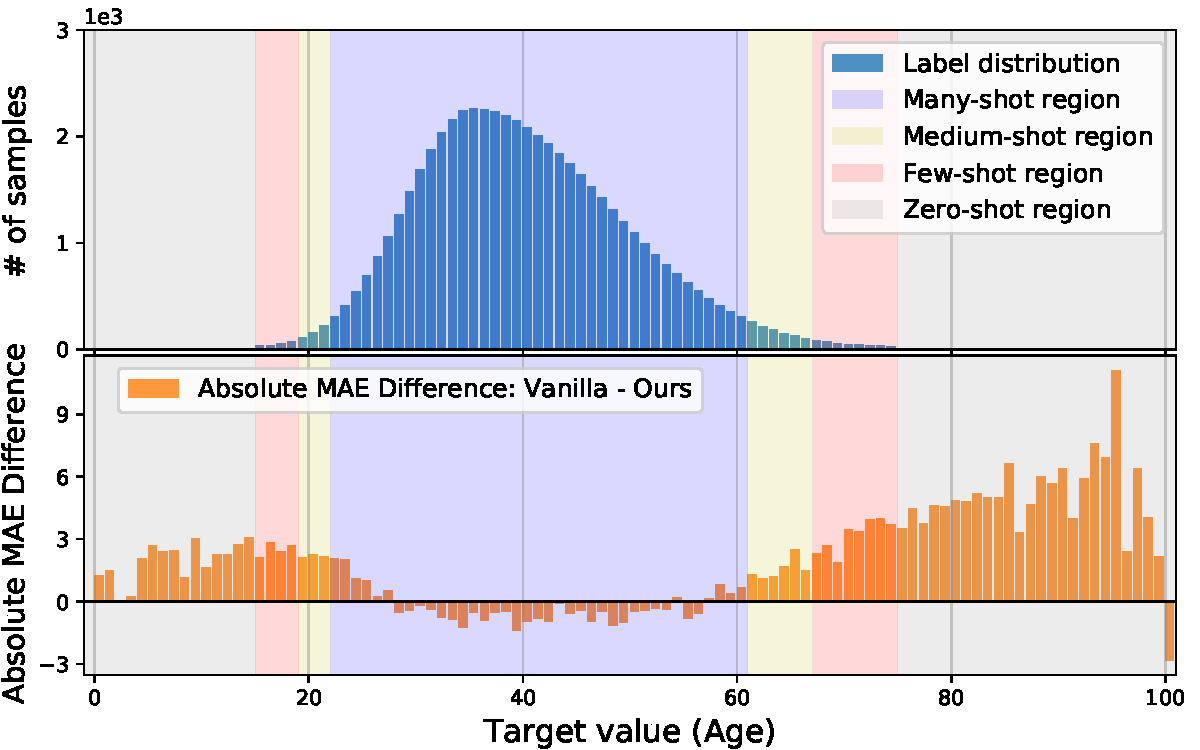
\includegraphics[width=0.7\linewidth]{images/interp_extrap_diff_peak1.pdf}
		\caption{MAE gains of LDS + FDS over the vanilla model.}
	\end{figure}
	\begin{itemize}
		\item Performance gains, esp. for extrapolation \& interpolation
	\end{itemize}
	\credit{Image}{yang2021delving}
\end{frame}

\begin{frame}{Skewed label distribution with two Gaussian peaks}
	\begin{figure}[h]
		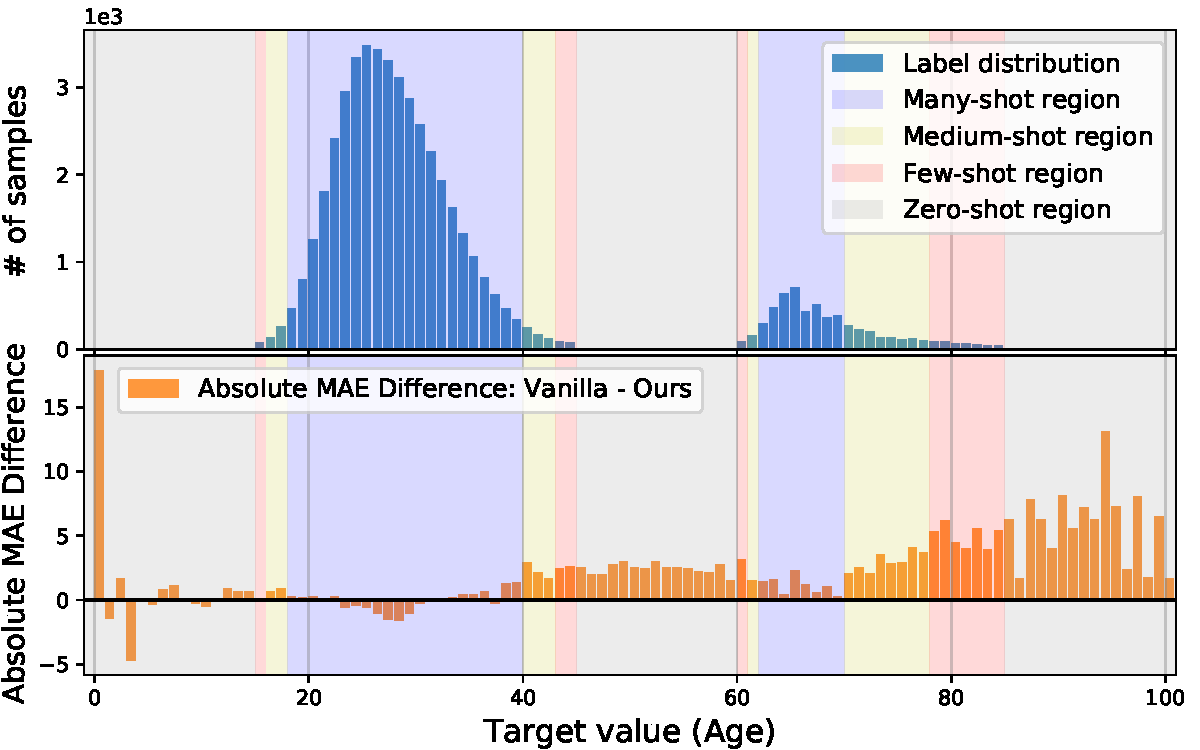
\includegraphics[width=0.7\linewidth]{images/interp_extrap_diff_peak2.pdf}
		\caption{MAE gains of LDS + FDS over the vanilla model.}
	\end{figure}
	\begin{itemize}
		\item Performance gains, esp. for extrapolation \& interpolation
	\end{itemize}
	\credit{Image}{yang2021delving}
\end{frame}

\begin{frame}{Skewed label distribution with three Gaussian peaks}
	\begin{figure}[h]
		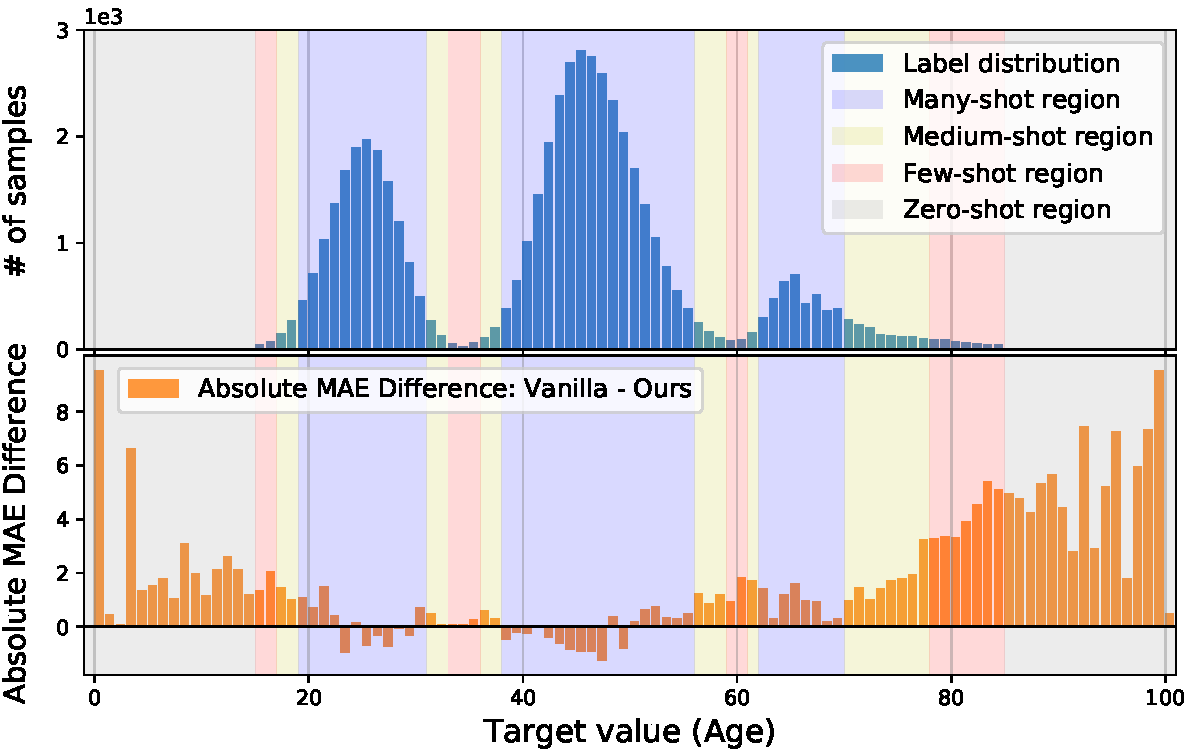
\includegraphics[width=0.7\linewidth]{images/interp_extrap_diff_peak3.pdf}
		\caption{MAE gains of LDS + FDS over the vanilla model.}
	\end{figure}
	\begin{itemize}
		\item Performance gains, esp. for extrapolation \& interpolation
	\end{itemize}
	\credit{Image}{yang2021delving}
\end{frame}

\begin{frame}{Skewed label distribution with four Gaussian peaks}
	\begin{figure}[h]
		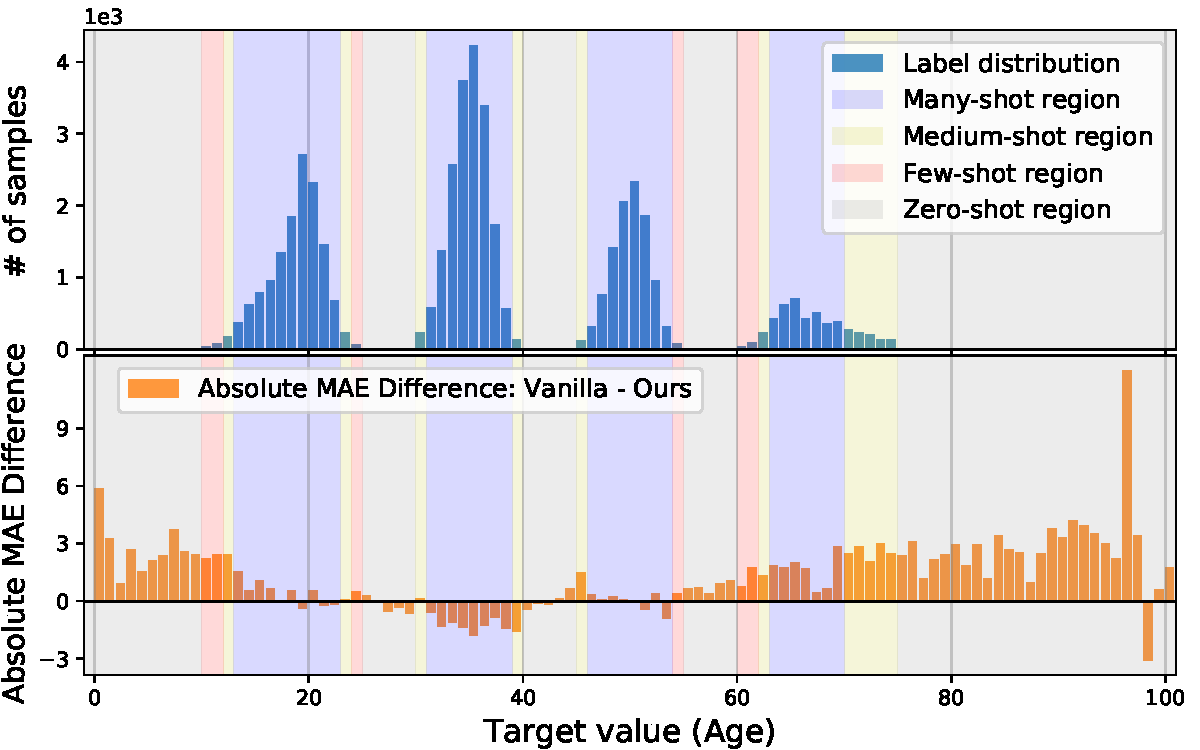
\includegraphics[width=0.7\linewidth]{images/interp_extrap_diff_peak4.pdf}
		\caption{MAE gains of LDS + FDS over the vanilla model.}
	\end{figure}
	\begin{itemize}
		\item Performance gains, esp. for extrapolation \& interpolation
	\end{itemize}
	\credit{Image}{yang2021delving}
\end{frame}

\begin{frame}{Skewed label distribution with two Gaussian peaks on IMDB-WIKI-DIR}
	\begin{table}[t]
		\setlength{\tabcolsep}{1.5pt}
		\small
		\begin{center}
			\resizebox{\textwidth}{!}{
				\begin{tabular}{l|cccc|cccc}
					\toprule[1.5pt]
					Metrics      & \multicolumn{4}{c|}{MAE~$\downarrow$}       & \multicolumn{4}{c}{GM~$\downarrow$}    \\ \midrule
					Shot         & All   & w/ data  & Interp. & Extrap.   & All   & w/ data  & Interp. & Extrap.   \\ \midrule\midrule
					\textsc{Vanilla}      & 11.72 & 9.32 & 16.13  & 18.19 & 7.44 & 5.33 &  14.41  & 16.74 \\ \midrule\midrule
					\textsc{Vanilla} + \textbf{\textsc{LDS}} &  10.54 &  8.31  &    14.14 & 17.38  & 6.50  & 4.67  & 12.13 & 15.36 \\[1.2pt]
					\textsc{Vanilla} + \textbf{\textsc{FDS}} & 11.40 & 8.97 & 15.83  & 18.01  & 7.18  & 5.12 & 14.02 & 16.48 \\[1.2pt]
					\textsc{Vanilla} + \textbf{\textsc{LDS}} + \textbf{\textsc{FDS}} & \textbf{10.27} & \textbf{8.11}  & \textbf{13.71} & \textbf{17.02}  & \textbf{6.33} & \textbf{4.55}  & \textbf{11.71}  & \textbf{15.13}  \\ \midrule\midrule
					\textsc{\textbf{Ours~(best)} vs. Vanilla}   & \textcolor{darkgreen}{\textbf{+1.45}} & \textcolor{darkgreen}{\textbf{+1.21}} & \textcolor{darkgreen}{\textbf{+2.42}} & \textcolor{darkgreen}{\textbf{+1.17}} & \textcolor{darkgreen}{\textbf{+1.11}} & \textcolor{darkgreen}{\textbf{+0.78}} & \textcolor{darkgreen}{\textbf{+2.70}} & \textcolor{darkgreen}{\textbf{+1.61}} \\
					\bottomrule[1.5pt]
				\end{tabular}
			}
		\end{center}
		\caption{Interpolation \& extrapolation results}
	\end{table}
	\begin{itemize}
		\item Best results by smoothing both label \& feature distributions
	\end{itemize}
	\credit{Table}{yang2021delving}
\end{frame}

\begin{frame}{Different skewed label distributions on IMDB-WIKI-DIR}
	\begin{table}[t]
		\setlength{\tabcolsep}{4.5pt}
		\label{table:appendix-skewed-dist}
		\small
		\begin{center}
			\resizebox{0.95\textwidth}{!}{
				\begin{tabular}{l|ccccccc|ccccccc}
					\toprule[1.5pt]
					Metrics      & \multicolumn{7}{c|}{MAE~$\downarrow$}       & \multicolumn{7}{c}{GM~$\downarrow$}    \\ \midrule
					Shot         & All   & Many & Med. & Few & Zero & Interp. & Extrap.   & All   & Many & Med. & Few & Zero & Interp. & Extrap.   \\ \midrule\midrule
					\multicolumn{9}{l}{\emph{\textbf{1 peak:}}} \\ \midrule
					\textsc{Vanilla}       & 11.20 & 6.05 & 11.43 & 14.76 & 22.67 & $-$ & 22.67 & 7.02 & \textbf{3.84} & 8.67 & 12.26 & 21.07 & $-$ & 21.07 \\ [1.2pt]
					\textsc{Vanilla} + \textbf{\textsc{LDS}}  & 10.09 & 6.26 & 9.91 & 12.12 & 19.37 & $-$ & 19.37 & 6.14 & 3.92 & 6.50 & 8.30 & 16.35 & $-$ & 16.35 \\[1.2pt]
					\textsc{Vanilla} + \textbf{\textsc{FDS}}  & 11.04 & \textbf{5.97} & 11.19 & 14.54 & 22.35 & $-$ & 22.35 & 6.96 & \textbf{3.84} & 8.54 & 12.08 & 20.71 & $-$ & 20.71 \\[1.2pt]
					\textsc{Vanilla} + \textbf{\textsc{LDS}} + \textbf{\textsc{FDS}}  & \textbf{10.00} & 6.28 & \textbf{9.66} & \textbf{11.83} & \textbf{19.21} & $-$ & \textbf{19.21} & \textbf{6.09} & 3.96 & \textbf{6.26} & \textbf{8.14} & \textbf{15.89} & $-$ & \textbf{15.89}  \\ \midrule\midrule
					\multicolumn{9}{l}{\emph{\textbf{2 peaks:}}} \\ \midrule
					\textsc{Vanilla}      & 11.72 & 6.83 & 11.78 & 15.35 & 16.86 & 16.13  & 18.19 & 7.44 & 3.61 & 8.06 & 12.94 &15.21&  14.41  & 16.74 \\ [1.2pt]
					\textsc{Vanilla} + \textbf{\textsc{LDS}} &  10.54  & 6.72 & 9.65 & 12.60 & 15.30&   14.14 & 17.38  & 6.50    & 3.65 & \textbf{5.65} & 9.30 & 13.20 & 12.13 & 15.36 \\[1.2pt]
					\textsc{Vanilla} + \textbf{\textsc{FDS}} & 11.40  & 6.69 & 11.02 & 14.85 & 16.61 & 15.83  & 18.01  & 7.18   & \textbf{3.50} & 7.49 & 12.73 & 14.86 & 14.02 & 16.48 \\[1.2pt]
					\textsc{Vanilla} + \textbf{\textsc{LDS}} + \textbf{\textsc{FDS}} & \textbf{10.27}  & \textbf{6.61} & \textbf{9.46} & \textbf{11.96} & \textbf{14.89} & \textbf{13.71} & \textbf{17.02}  & \textbf{6.33}   & 3.54 & 5.68 & \textbf{8.80} & \textbf{12.83} & \textbf{11.71}  & \textbf{15.13}  \\ \midrule\midrule
					\multicolumn{9}{l}{\emph{\textbf{3 peaks:}}} \\ \midrule
					\textsc{Vanilla}      & 9.83  & 7.01 & 9.81 & 11.93 & 20.11 & $-$ & 20.11 & 6.04 & 3.93 & 6.94 & 9.84 & 17.77 & $-$ & 17.77 \\ [1.2pt]
					\textsc{Vanilla} + \textbf{\textsc{LDS}} & 9.08 & \textbf{6.77} & 8.82 & 10.48 & 18.43 & $-$ & 18.43 & \textbf{5.35} & \textbf{3.78} & 5.63 & 7.49 & 15.46 & $-$ & 15.46 \\[1.2pt]
					\textsc{Vanilla} + \textbf{\textsc{FDS}} & 9.65 & 6.88 & 9.58 & 11.75 & 19.80 & $-$ & 19.80 & 5.86 & 3.83 & 6.68 & 9.48 & 17.43 & $-$ & 17.43 \\[1.2pt]
					\textsc{Vanilla} + \textbf{\textsc{LDS}} + \textbf{\textsc{FDS}} & \textbf{8.96} & 6.88 & \textbf{8.62} & \textbf{10.08} & \textbf{17.76} & $-$ & \textbf{17.76} & 5.38  & 3.90 & \textbf{5.61} & \textbf{7.36} & \textbf{14.65} & $-$ & \textbf{14.65}  \\ \midrule\midrule
					\multicolumn{9}{l}{\emph{\textbf{4 peaks:}}} \\ \midrule
					\textsc{Vanilla}      & 9.49 & 7.23 & 9.73 & 10.85 & 12.16 & 8.23 & 18.78 & 5.68 & 3.45 & 6.95 & 8.20 & 9.43 & 6.89 & 16.02 \\ [1.2pt]
					\textsc{Vanilla} + \textbf{\textsc{LDS}} & 8.80 & \textbf{6.98} & 8.26 & 10.07 & 11.26 & 8.31 & \textbf{16.22} & 5.10 & \textbf{3.33} & \textbf{5.07} & 7.08 & 8.47 & 6.66 & \textbf{12.74} \\[1.2pt]
					\textsc{Vanilla} + \textbf{\textsc{FDS}} & 9.28 & 7.11 & 9.16 & 10.88 & 11.95 & 8.30 & 18.11 & 5.49 & 3.36 & 6.35 & 8.15 & 9.21 & 6.82 & 15.30 \\[1.2pt]
					\textsc{Vanilla} + \textbf{\textsc{LDS}} + \textbf{\textsc{FDS}} & \textbf{8.76} & 7.07 & \textbf{8.23} & \textbf{9.54} & \textbf{11.13} & \textbf{8.05} & 16.32 & \textbf{5.05} & 3.36 & \textbf{5.07} & \textbf{6.56} & \textbf{8.30} & \textbf{6.34} & 13.10  \\ 
					\bottomrule[1.5pt]
				\end{tabular}
			}
		\end{center}
	\end{table}
	\credit{Table}{yang2021delving}
\end{frame}

\section{References}
\begin{frame}[noframenumbering,plain]%[allowframebreaks]
\frametitle{References}
\printbibliography
\end{frame}

\end{document}